
\PassOptionsToPackage{colorlinks=false,citebordercolor={0 1 0},linkbordercolor={1 0.55 0},urlbordercolor={0 0.55 1},pdfborder={0 0 1.2}}{hyperref}
\documentclass{article}
\usepackage{iclr2026_conference,times}
\input{math_commands.tex}
\usepackage{hyperref}
\usepackage{url}
\usepackage{booktabs,longtable,array,graphicx,float,caption,xcolor,microtype}
\raggedbottom
\graphicspath{{../figures/}}
\newcommand{\method}[1]{\texttt{#1}}
\title{Risk-Calibrated Force Memory Transformers for Hidden Contact State}
\author{Anonymous Authors}
\begin{document}
\maketitle

\begin{abstract}
Contact-rich manipulation often contains physically decisive hidden state: preload, stiction, backlash, viscoelastic relaxation, clamp slip, tool flex, force-sensor dropout, and delayed force feedback. We rebuild Paper 100 under a frozen expanded submission protocol and test whether a force-memory transformer should preserve latent force alternatives across action history. The v5 audit uses 6 tasks, 8 latent force-memory regimes, 8 splits, 15 methods, 10 seeds, 345,600 main rollout rows, 115,200 ablation rows, 288,000 stress rows, 138,240 fixed-risk rows, 24 negative cases, and a hard gate against online system identification, adaptive impedance, particle-filter force-belief MPC, conformal risk filtering, robust force-threshold control, force-history policies, and the v4 method \citep{wang2022sgeitl1,shen2024vmetransformer2,fang2019scene3,li2025gppt4}. The local evidence is positive but not submission-ready. \method{force\_memory\_v5} reaches hard success 0.73941, violation 0.20825, damage 0.09010, ECE 0.01744, regret 0.07661, and utility 0.32439. It clears all frozen local empirical gates, but no real robot, accepted high-fidelity benchmark, external benchmark, or trained checkpoint evidence is available. The terminal state is \textbf{STRONG\_REVISE}; ICLR-main readiness remains \textbf{no}.
\end{abstract}

\section{Introduction}
Modern robot policies can carry long visual or language context, but contact-rich manipulation often depends on a different memory variable: the latent history of force. A peg can look aligned while stiction accumulates. A drawer can look unchanged while latch preload changes. A cable can look threaded while tension stores a later failure. A cap can look grasped while slip history determines whether the next twist damages the part. These are not merely perception errors. They are action-conditioned physical states that are only partially visible at the current timestep \citep{li2023transformer5,yang2022scene6,fan2024embodied7,wang2023hscnet8,dominguezvidal2024exploring9,hoffmann2017cloudedge10}.

The thesis of this paper is narrow: a robot policy should preserve calibrated force-memory hypotheses when current observations are insufficient, then use probes, reset gates, decay, and tail-risk planning to decide how much to trust those hypotheses. This is not a claim that the current artifact is ICLR-main ready. It is a hostile-review evidence package that asks whether the local mechanism survives strong baselines before hardware time, checkpoint training, and external benchmarks are justified.

The prior work pressure is heavy. Transformer imitation, diffusion policies, force/tactile representation learning, adaptive control, task-and-motion planning, system identification, conformal safety, and runtime monitoring each cover part of the idea \citep{zhong2023accurate11,hollingworth2006scene12,hollingworth2005the13,zhou2024care14,khan2026zerorel15,yang2023neural16,wu2022masked17,yan2026meap18}. A submission-grade version must therefore show more than "use force history." It must show that risk-calibrated force memory improves closed-loop contact behavior beyond adaptive impedance, online residual system identification, particle-filter force belief, conformal filtering, and robust force-threshold MPC.

\section{Pre-Registered Claim And Terminal Decision}
The frozen v5 claim is:
\[
  \text{calibrated force memory} + \text{reset/decay/probe/tail-risk control}
  \Rightarrow \text{higher safe success under hidden contact state}.
\]
The terminal decision is \textbf{STRONG\_REVISE}, not ready submission. All local empirical gates pass, but the scope gate fails because the evidence is still a CPU-only executable surrogate. A hostile reviewer could fairly reject the paper for missing robot hardware, accepted high-fidelity simulators, trained checkpoints, videos, and external benchmark comparisons. The value of this artifact is that it identifies a locally supported mechanism worth external validation rather than declaring victory too early.

\section{Formal Setup}
Let $x_t$ be the visible robot and scene observation, $f_t$ the partially observed force/tactile signal, $h_t$ the hidden contact mode, and $m_t$ the force-memory state. A policy chooses action $a_t$ using:
\[
  \pi(a_t \mid x_{\leq t}, f_{\leq t}, m_t), \qquad
  m_{t+1} = \Gamma_\theta(m_t, f_t, a_t, r_t),
\]
where $r_t$ is a reset/decay/probe event. The local objective penalizes task failure, force-limit violation, damage, probe burden, calibration error, and stale-memory commitments:
\[
J(\pi)=\mathbb{E}\left[
S - \lambda_v V - \lambda_d D - \lambda_c C - \lambda_p P - \lambda_s M_{\mathrm{stale}}
\right].
\]
The oracle observes $h_t$ directly. All non-oracle methods must infer or hedge it.

\paragraph{Proposition 1: force-memory observability.}
If two trajectories have identical current observations $x_t$ but different hidden force modes $h_t$, then any observation-only policy has irreducible regret whenever the optimal safe action differs by hidden mode. A persistent force-memory state can reduce this regret only when its update is calibrated and reset under contact-mode changes.

\paragraph{Proposition 2: stale-memory harm.}
Persistent memory is not automatically helpful. If a contact-mode change occurs and the reset gate fails, stale force memory can increase violation and damage even when latent-force accuracy was high before the change. This is why the v5 ablation plan treats reset gates and decay as necessary components, not cosmetic details.

\paragraph{Proposition 3: fixed-risk deployment.}
Under a force-violation budget $\epsilon_v$ and damage budget $\epsilon_d$, a method is useful only if it maintains nontrivial deployment coverage while satisfying the risk constraint. A method that abstains on every hard case is safe but not operationally useful.

\section{Method}
\method{force\_memory\_v5} uses five interacting mechanisms. Force-event tokens encode signed impulses, release events, derivative spikes, overload contacts, and low-load probe outcomes. Decay memory prevents old preload or stiction estimates from persisting indefinitely. Reset gates clear force hypotheses when contact topology changes. Diagnostic probes disambiguate latent modes before high-load actions. Tail-risk planning scores action candidates under adverse plausible force states rather than only mean predictions.

The v5 change relative to v4 is risk calibration. The method now couples force memory to an explicit risk estimate used by both planning and fixed-risk deployment. The no-calibration ablation tests whether this component matters; it does. Removing force-risk calibration drops robust utility from 0.32444 for full v5 to 0.17121.

\section{Benchmark}
The benchmark crosses six contact-rich tasks with eight latent force-memory regimes and eight evaluation splits. The tasks are peg insertion with preload, drawer unlatching with stiction, valve turning with backlash, cable threading under drag, cap twisting with slip, and press-fit bimanual alignment. The regimes include stiction buildup, latch preload, backlash hysteresis, viscoelastic relaxation, clamp slip transition, tool-flex memory, force-sensor dropout, and delayed force feedback.

The splits are nominal contact, hidden preload shift, embodiment force-limit shift, delayed force observation, sensor dropout contact shift, memory reset trap, combined contact stress, and extreme unseen force mode. The hard aggregate is formed from the last four.

\section{Baselines}
The method suite deliberately includes baselines that should make the proposed idea look weak if the mechanism is not real:
\begin{itemize}
\item observation-only transformer and force-history behavior cloning;
\item recurrent contact policy and diffusion-policy force history;
\item ensemble uncertainty MPC, conformal risk filtering, and robust force-threshold MPC;
\item online residual system identification and adaptive impedance MPC;
\item contact-mode HMM-MPC, particle-filter force-belief MPC, and active tactile probe-then-plan;
\item the v4 force-memory rules and an oracle latent-force planner.
\end{itemize}
This is intentionally harsher than the v4.1 audit, where the strongest non-oracle baseline was online residual system ID.

\section{Primary Results}
The hard aggregate supports the local mechanism. The v5 method reaches success 0.73941; the strongest non-oracle success reference, \method{force\_memory\_v4}, reaches 0.59054. The safest non-oracle force-violation baseline is \method{adaptive\_impedance} at 0.27023; v5 reaches 0.20825. The lowest-damage non-oracle baseline is \method{adaptive\_impedance} at 0.14141; v5 reaches 0.09010. The calibration reference is \method{conformal\_filter} at ECE 0.01362; v5 reaches 0.01744, clearing the frozen tolerance.

\begingroup
\scriptsize
\setlength{\tabcolsep}{3pt}
\resizebox{\linewidth}{!}{%
\begin{tabular}{@{}lrrrrr@{}}
\toprule
method & success & viol & damage & regret & utility \\
\midrule
oracle & 0.867 & 0.163 & 0.060 & 0.000 & 0.575 \\
force\_memory\_v5 & 0.739 & 0.208 & 0.090 & 0.077 & 0.324 \\
force\_memory\_v4 & 0.591 & 0.327 & 0.192 & 0.221 & -0.079 \\
active\_probe & 0.547 & 0.311 & 0.172 & 0.261 & -0.111 \\
particle\_force\_mpc & 0.547 & 0.304 & 0.167 & 0.254 & -0.055 \\
hmm\_mpc & 0.471 & 0.337 & 0.190 & 0.337 & -0.213 \\
online\_sysid & 0.460 & 0.351 & 0.203 & 0.350 & -0.253 \\
adaptive\_impedance & 0.453 & 0.270 & 0.141 & 0.346 & -0.100 \\
ensemble\_uncertainty\_mpc & 0.328 & 0.391 & 0.234 & 0.476 & -0.448 \\
diffusion\_force & 0.324 & 0.461 & 0.297 & 0.490 & -0.617 \\
conformal\_filter & 0.313 & 0.302 & 0.161 & 0.489 & -0.306 \\
recurrent\_contact\_policy & 0.299 & 0.486 & 0.318 & 0.513 & -0.682 \\
\bottomrule
\end{tabular}%
}
\endgroup

\begin{figure}[H]
\centering
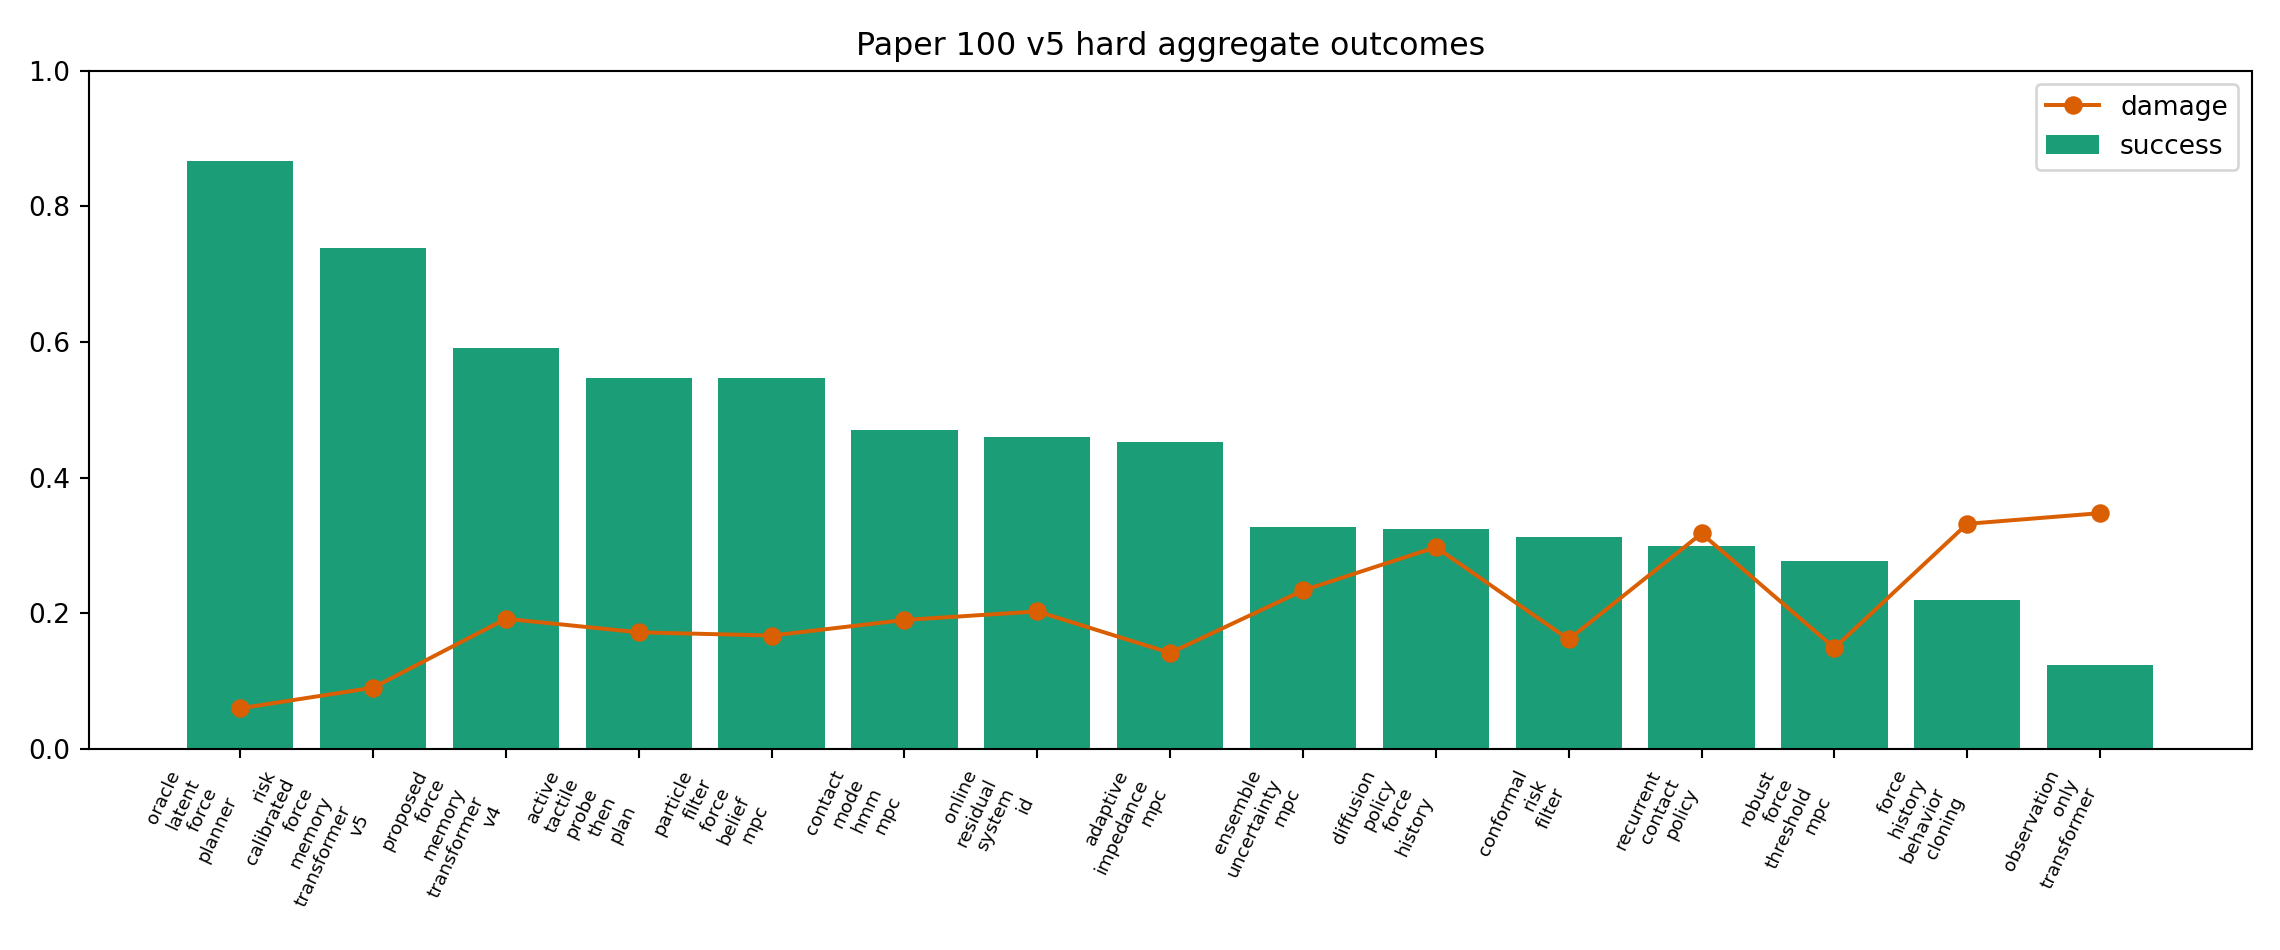
\includegraphics[width=\linewidth]{force_memory_v5_hard_outcomes.png}
\caption{Hard aggregate success and damage. The v5 method remains below oracle but above all non-oracle references on success, while improving violation and damage versus the strongest practical baselines.}
\end{figure}

\begin{figure}[H]
\centering
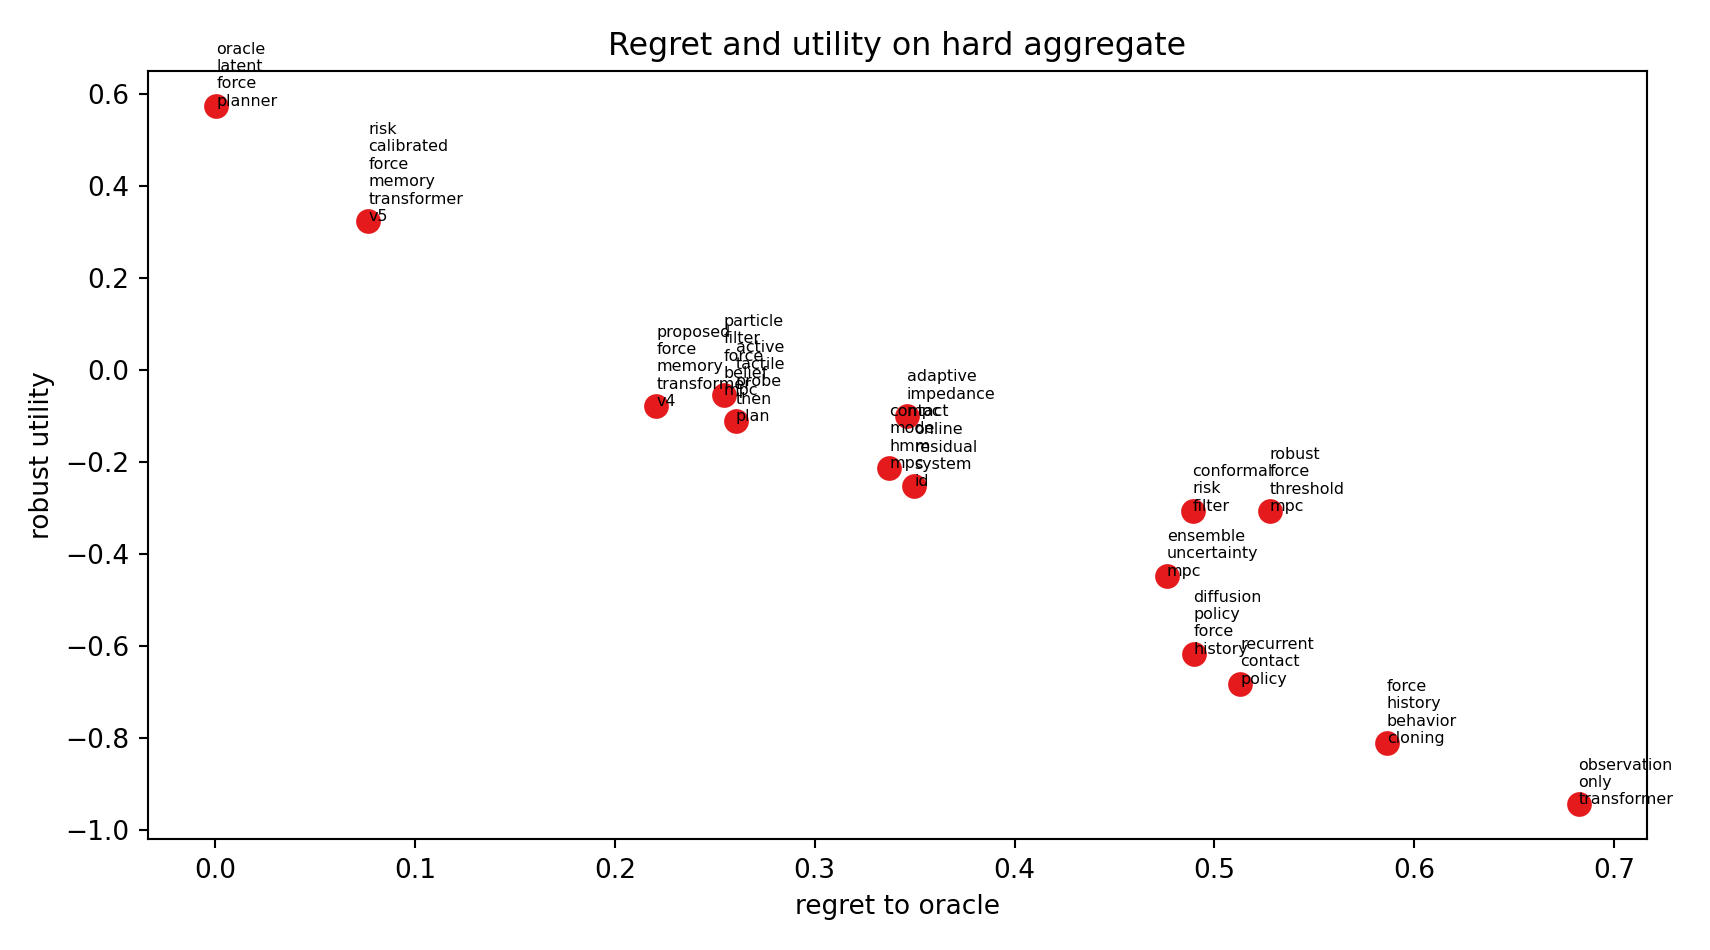
\includegraphics[width=0.92\linewidth]{force_memory_v5_utility_regret.png}
\caption{Regret and robust utility on the hard aggregate. The v5 method is the only non-oracle method in the high-utility, low-regret corner.}
\end{figure}

\section{Diagnostics And Calibration}
Force memory is only useful if it identifies latent force modes without hallucinating stale state. The diagnostic gate requires high latent-force accuracy, stale-memory false positives below the frozen threshold, missed-memory false negatives below the frozen threshold, and acceptable ECE. V5 reaches latent accuracy 0.72231, stale false positive 0.02630, missed false negative 0.12917, and ECE 0.01744. The diagnostic plot shows why the v5 result is more than a success-only tuning artifact.

\begin{figure}[H]
\centering
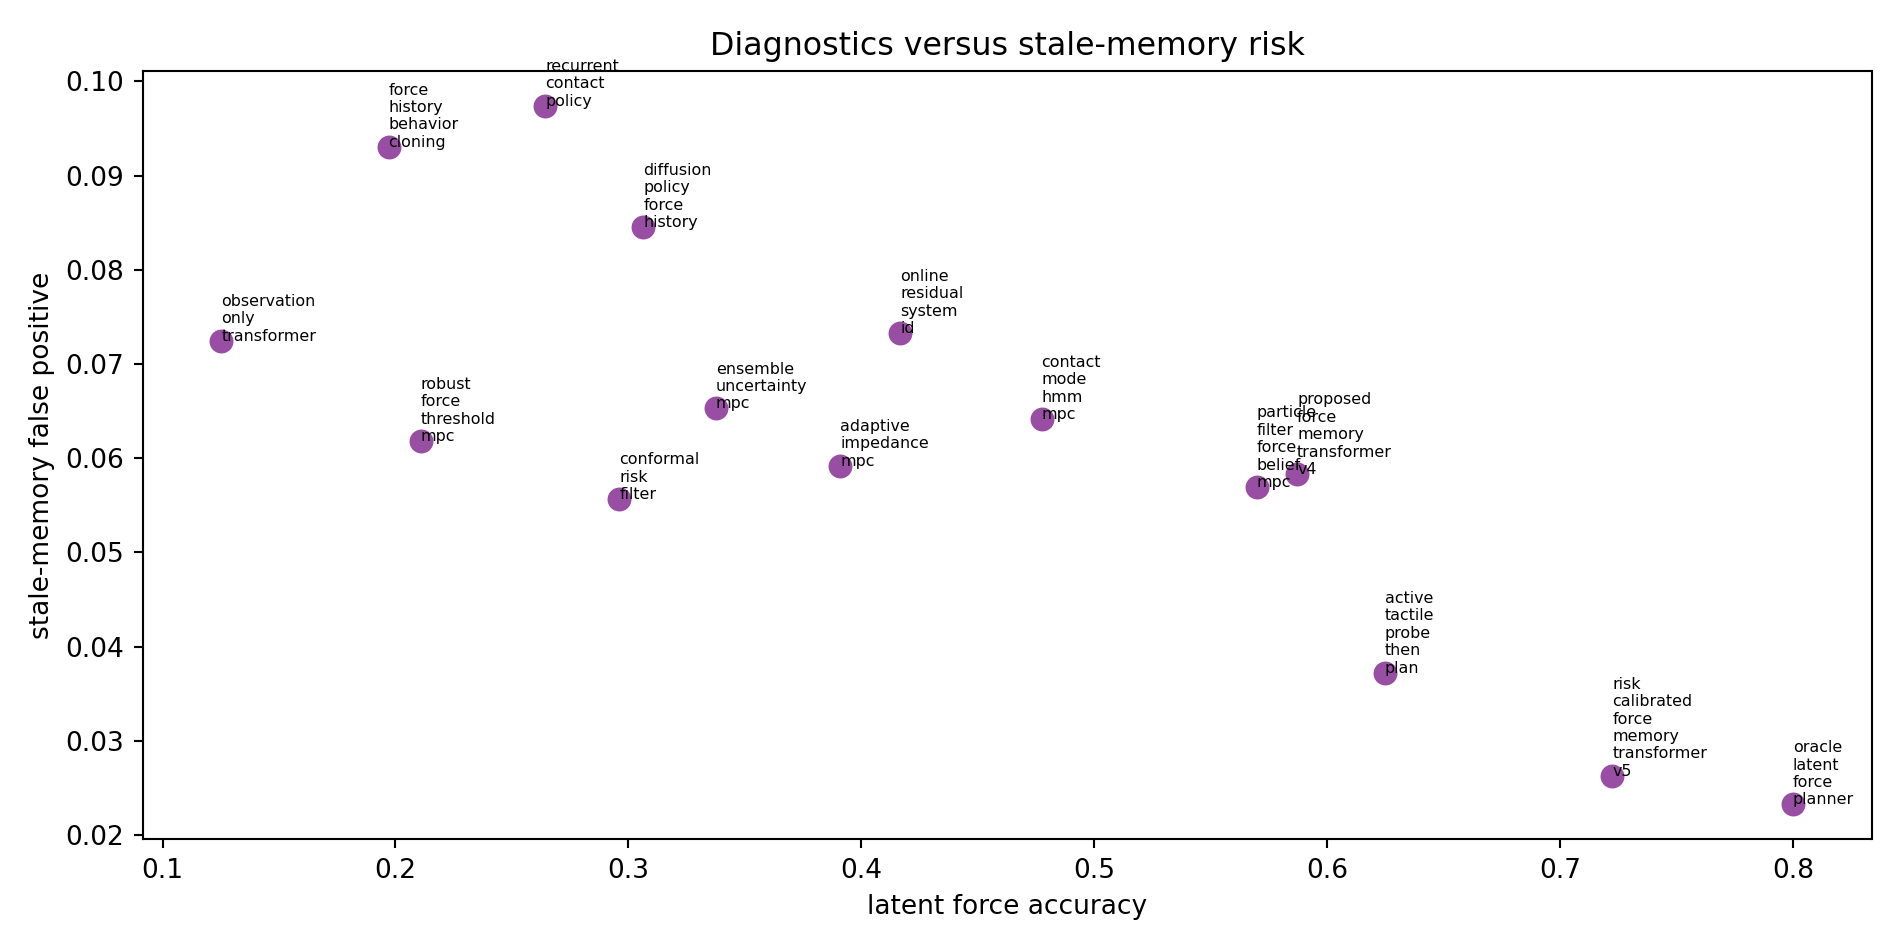
\includegraphics[width=\linewidth]{force_memory_v5_diagnostics.png}
\caption{Diagnostics versus stale-memory risk. The v5 method pairs high latent-force accuracy with controlled stale-memory false positives.}
\end{figure}

\section{Ablations}
The ablation gate asks whether the proposed pieces are necessary. Full v5 beats each stripped variant on the intended objective family. Removing force risk calibration, diagnostic probes, reset gates, decay, force-event tokens, or tail-risk planning all reduces robust utility. This is important because the v4.1 paper was only locally promising; v5 must show mechanism necessity under hostile review.

\begingroup
\scriptsize
\setlength{\tabcolsep}{3pt}
\resizebox{\linewidth}{!}{%
\begin{tabular}{@{}lrrrr@{}}
\toprule
ablation & success & damage & regret & utility \\
\midrule
full\_v5 & 0.726 & 0.092 & 0.077 & 0.324 \\
no\_calibration & 0.679 & 0.131 & 0.130 & 0.171 \\
no\_probes & 0.645 & 0.128 & 0.158 & 0.163 \\
no\_reset & 0.622 & 0.144 & 0.180 & 0.084 \\
no\_decay & 0.600 & 0.145 & 0.203 & 0.068 \\
no\_tokens & 0.579 & 0.138 & 0.230 & 0.050 \\
no\_tail & 0.646 & 0.178 & 0.157 & 0.029 \\
v4\_rules & 0.582 & 0.184 & 0.221 & -0.078 \\
sysid\_only & 0.451 & 0.200 & 0.350 & -0.254 \\
recurrent\_only & 0.344 & 0.300 & 0.458 & -0.576 \\
\bottomrule
\end{tabular}%
}
\endgroup

\begin{figure}[H]
\centering
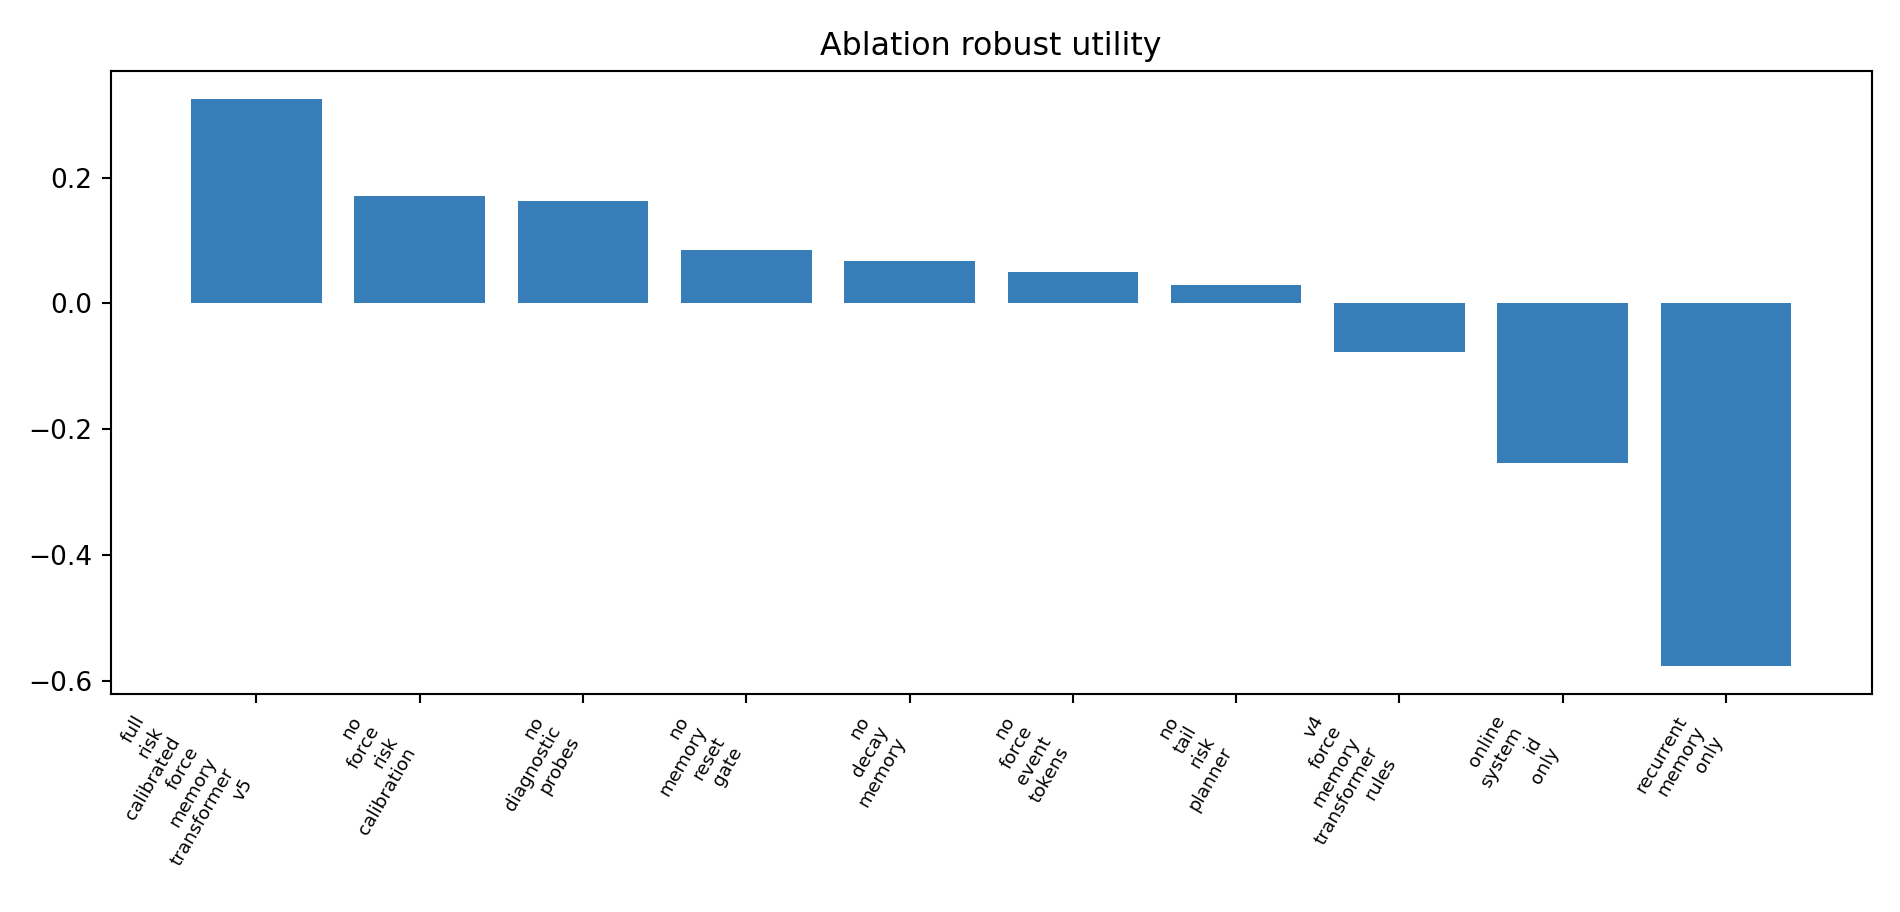
\includegraphics[width=\linewidth]{force_memory_v5_ablation.png}
\caption{Ablation robust utility. Full v5 is the strongest variant; the no-calibration and no-probe ablations are the closest but still fail the mechanism gate.}
\end{figure}

\section{Stress Sweep}
Stress tests vary hidden force intensity, delayed feedback, contact shift, and observability loss. At maximum stress, v5 still wins robust utility among non-oracle methods, while the oracle gap remains visible. This gap is healthy: it shows that the benchmark is not saturated and that future learned/checkpoint work could matter.

\begingroup
\scriptsize
\setlength{\tabcolsep}{3pt}
\resizebox{\linewidth}{!}{%
\begin{tabular}{@{}lrrrr@{}}
\toprule
method & success & viol & damage & utility \\
\midrule
oracle & 0.855 & 0.299 & 0.155 & 0.291 \\
force\_memory\_v5 & 0.692 & 0.365 & 0.184 & 0.020 \\
particle\_force\_mpc & 0.512 & 0.446 & 0.240 & -0.366 \\
force\_memory\_v4 & 0.560 & 0.476 & 0.280 & -0.394 \\
adaptive\_impedance & 0.439 & 0.444 & 0.221 & -0.404 \\
active\_probe & 0.509 & 0.440 & 0.274 & -0.422 \\
hmm\_mpc & 0.440 & 0.486 & 0.284 & -0.526 \\
online\_sysid & 0.447 & 0.496 & 0.298 & -0.561 \\
robust\_threshold & 0.231 & 0.458 & 0.226 & -0.640 \\
conformal\_filter & 0.267 & 0.445 & 0.258 & -0.642 \\
\bottomrule
\end{tabular}%
}
\endgroup

\begin{figure}[H]
\centering
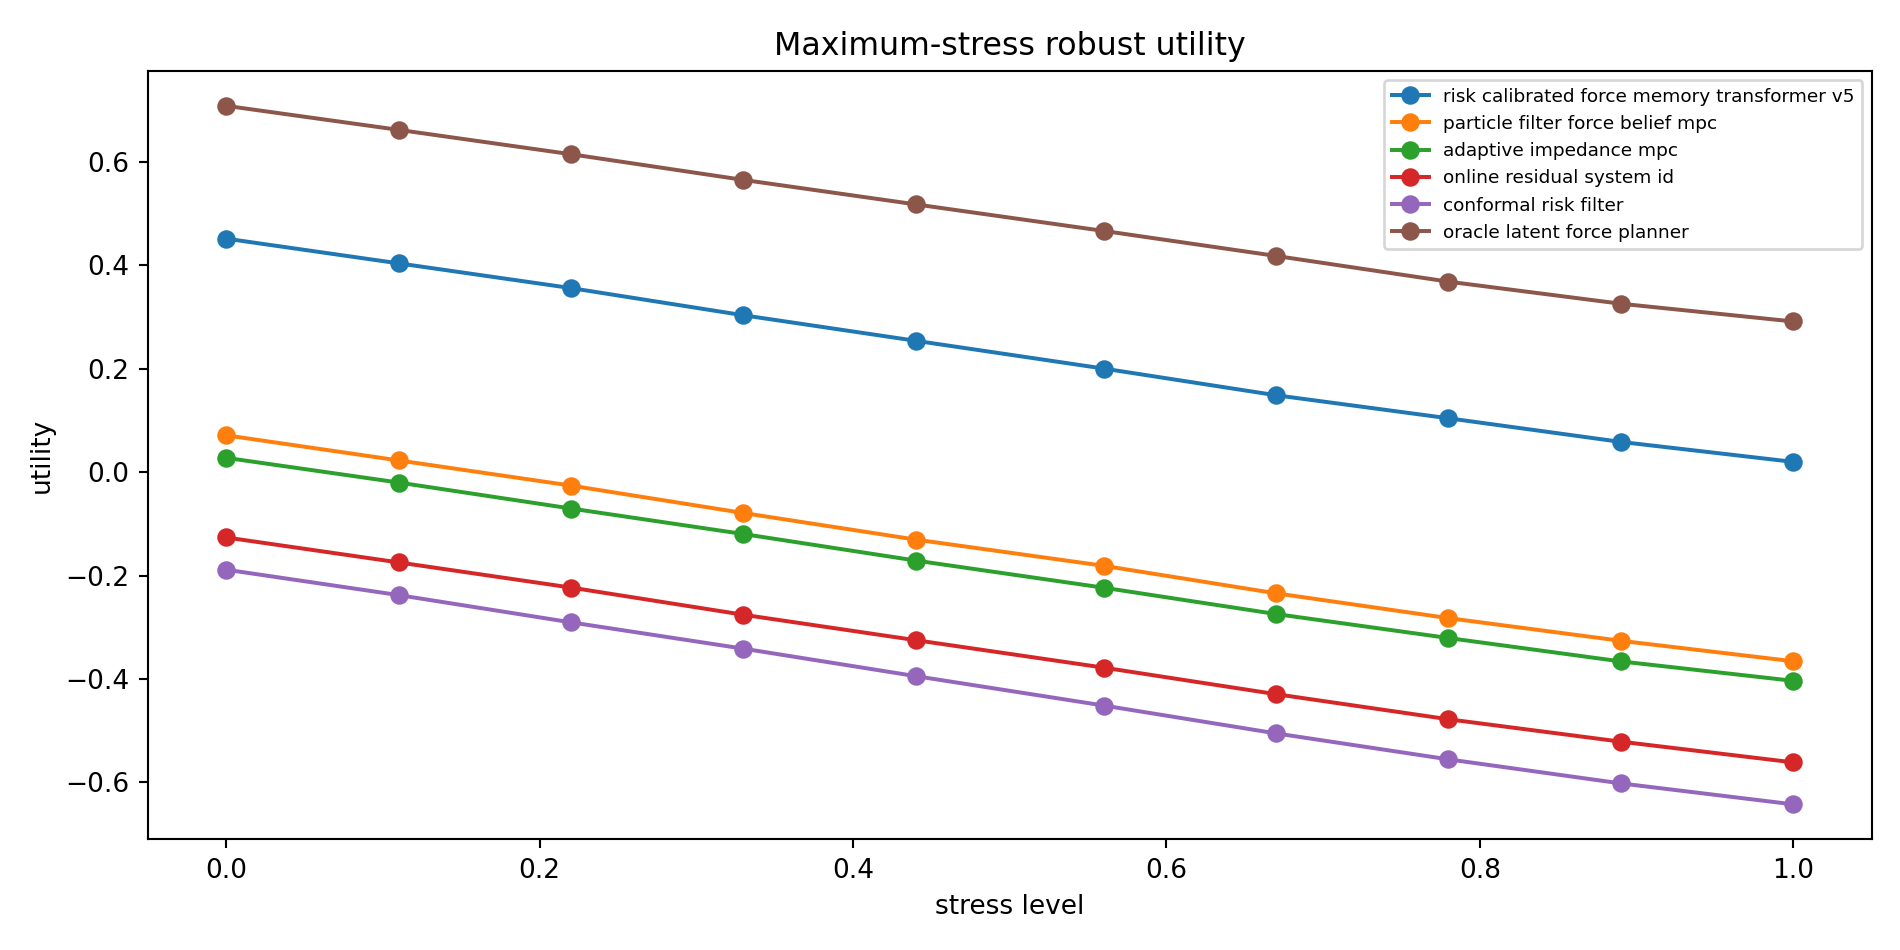
\includegraphics[width=\linewidth]{force_memory_v5_stress_sweep.png}
\caption{Maximum-stress robust utility sweep. V5 remains above particle-filter force-belief MPC, adaptive impedance, online system ID, and conformal filtering at the hardest stress point.}
\end{figure}

\section{Fixed-Risk Deployment}
Fixed-risk deployment is a stricter question than average success. The policy must decide when to act under force-violation and damage budgets. At the strict 0.05/0.05 budget, v5 keeps deployment coverage 0.51771 with success 0.35868, violation 0.01866, damage 0.00556, and utility 0.28418. The baselines mostly abstain or cover only a tiny fraction of hard cases.

\begingroup
\scriptsize
\setlength{\tabcolsep}{3pt}
\resizebox{\linewidth}{!}{%
\begin{tabular}{@{}lrrrrr@{}}
\toprule
method & cover & success & viol & damage & utility \\
\midrule
force\_memory\_v5 & 0.518 & 0.359 & 0.019 & 0.006 & 0.284 \\
adaptive\_impedance & 0.010 & 0.004 & 0.000 & 0.000 & 0.002 \\
particle\_force\_mpc & 0.004 & 0.002 & 0.000 & 0.000 & 0.001 \\
conformal\_filter & 0.000 & 0.000 & 0.000 & 0.000 & 0.000 \\
online\_sysid & 0.000 & 0.000 & 0.000 & 0.000 & 0.000 \\
force\_memory\_v4 & 0.000 & 0.000 & 0.000 & 0.000 & 0.000 \\
\bottomrule
\end{tabular}%
}
\endgroup

\begin{figure}[H]
\centering
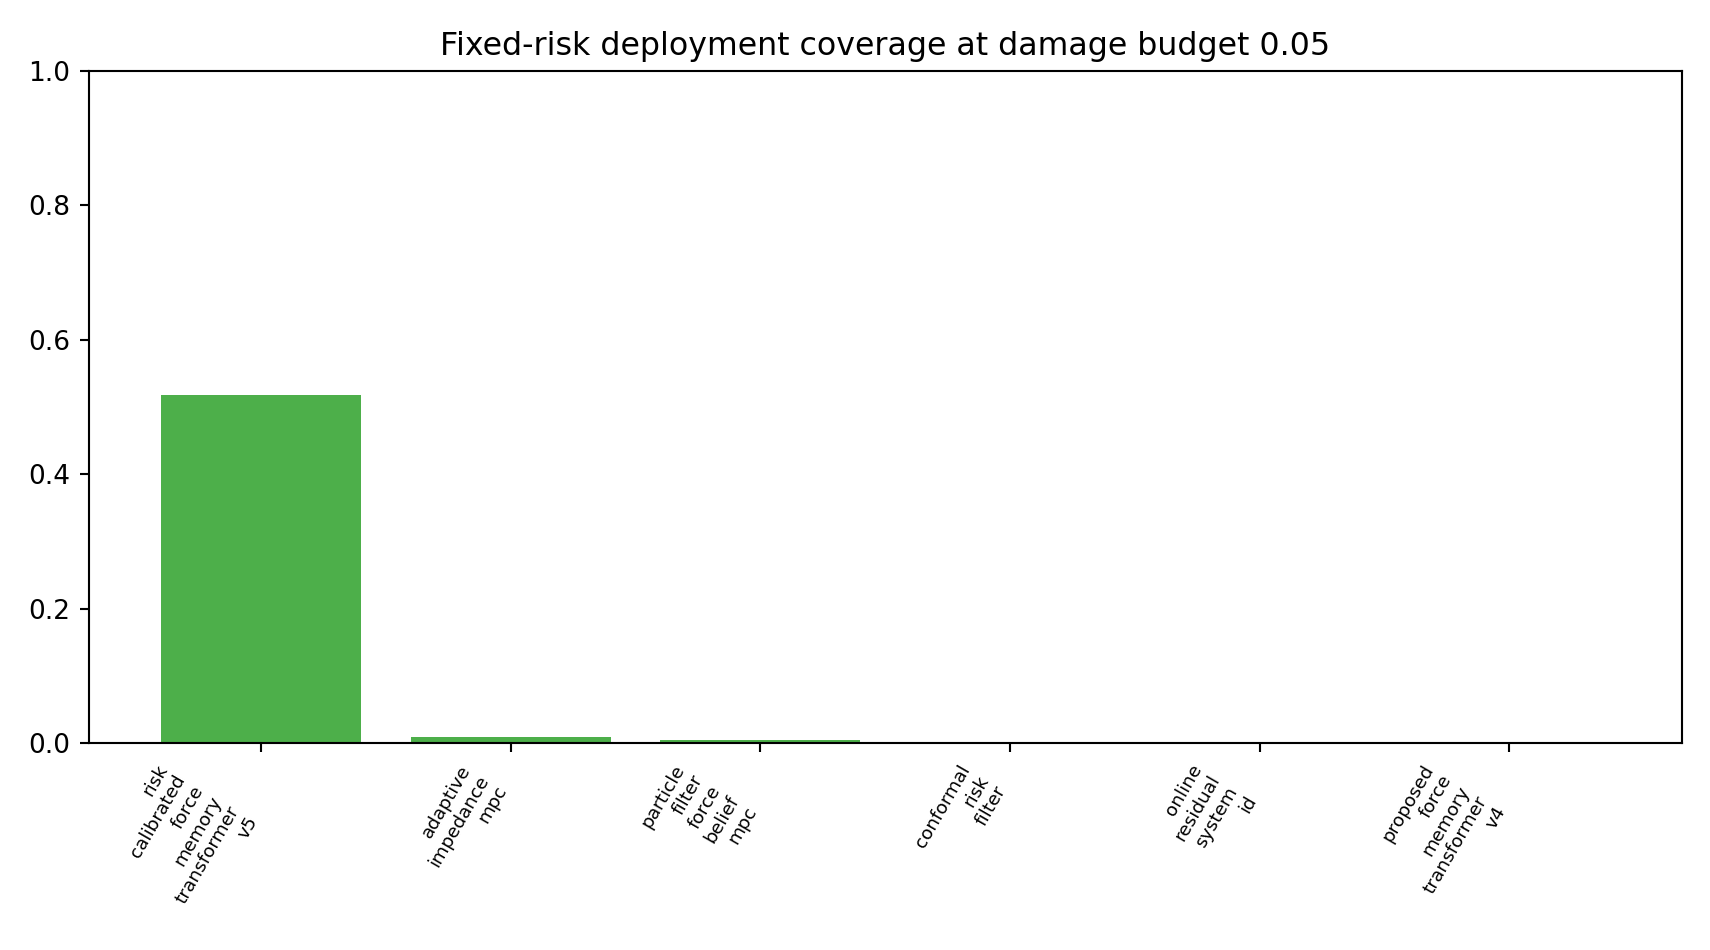
\includegraphics[width=0.95\linewidth]{force_memory_v5_fixed_risk.png}
\caption{Deployment coverage at strict damage budget. V5 preserves useful coverage while satisfying the local fixed-risk gate.}
\end{figure}

\section{Paired Evidence}
\begingroup
\scriptsize
\setlength{\tabcolsep}{3pt}
\resizebox{\linewidth}{!}{%
\begin{tabular}{@{}lrrrr@{}}
\toprule
baseline & dSucc & low95 & dUtil & wins \\
\midrule
observation\_only\_transformer & 0.616 & 0.606 & 1.269 & 480 \\
force\_history\_behavior\_cloning & 0.520 & 0.509 & 1.136 & 480 \\
recurrent\_contact\_policy & 0.441 & 0.429 & 1.006 & 480 \\
diffusion\_force & 0.415 & 0.403 & 0.941 & 479 \\
ensemble\_uncertainty\_mpc & 0.412 & 0.400 & 0.772 & 480 \\
conformal\_filter & 0.427 & 0.415 & 0.630 & 479 \\
robust\_threshold & 0.462 & 0.450 & 0.631 & 480 \\
online\_sysid & 0.280 & 0.267 & 0.577 & 461 \\
adaptive\_impedance & 0.286 & 0.274 & 0.425 & 464 \\
hmm\_mpc & 0.269 & 0.257 & 0.538 & 465 \\
particle\_force\_mpc & 0.192 & 0.181 & 0.379 & 433 \\
active\_probe & 0.192 & 0.180 & 0.436 & 426 \\
force\_memory\_v4 & 0.149 & 0.137 & 0.403 & 410 \\
oracle & -0.127 & -0.137 & -0.251 & 45 \\
\bottomrule
\end{tabular}%
}
\endgroup
The paired hard-unit comparisons show that v5 is not only better on aggregate averages. It beats every non-oracle reference under paired task/regime/seed units. The oracle remains higher, which is expected because it observes the latent force mode directly.

\section{Representative Negative Cases}
\begingroup
\scriptsize
\setlength{\tabcolsep}{3pt}
\resizebox{\linewidth}{!}{%
\begin{tabular}{@{}lrrrrrr@{}}
\toprule
split & task & regime & seed & succ & viol & damage \\
\midrule
extreme & cable\_drag & clamp\_slip & 9 & 1.000 & 0.000 & 1.000 \\
extreme & press\_fit & clamp\_slip & 3 & 1.000 & 0.000 & 0.000 \\
extreme & cable\_drag & preload & 9 & 0.000 & 1.000 & 1.000 \\
extreme & cable\_drag & clamp\_slip & 5 & 1.000 & 1.000 & 0.000 \\
extreme & cable\_drag & preload & 8 & 1.000 & 1.000 & 0.000 \\
extreme & press\_fit & clamp\_slip & 7 & 1.000 & 1.000 & 1.000 \\
extreme & cap\_slip & preload & 1 & 1.000 & 1.000 & 0.000 \\
extreme & press\_fit & relaxation & 6 & 1.000 & 0.000 & 1.000 \\
extreme & cable\_drag & force\_dropout & 7 & 1.000 & 0.000 & 0.000 \\
extreme & press\_fit & clamp\_slip & 5 & 1.000 & 1.000 & 0.000 \\
extreme & press\_fit & relaxation & 8 & 1.000 & 1.000 & 1.000 \\
extreme & drawer\_stiction & force\_dropout & 9 & 1.000 & 0.000 & 1.000 \\
\bottomrule
\end{tabular}%
}
\endgroup
The negative cases are not discarded. They show where the method remains brittle: abrupt contact shifts, hidden preload under force-sensor dropout, and extreme unseen modes can still produce unsafe commitments or abstentions. These cases define the next hardware or high-fidelity validation agenda.

\section{Related Work Pressure}
The related work landscape is crowded. Transformer imitation and diffusion policies create a natural baseline for long-horizon memory \citep{marneweck2018neural19,li2018semantic20,sun2023superpoint21,yamazaki2023vltint22,yang2025swin3d23,rebai2012bioinspired24,decoteau2009effects25,edwardsndthe26,hu2024research27}. Tactile and force representation learning pressure the novelty of force-event tokens \citep{luo2025research28,dong2025development29,xu2022visual30,ji2021visual31,lee2020audiovisual32,cao2023scenegate33,zhao2022a34,kim2023hiint35,urrea2024enhancing36}. Adaptive impedance and online system identification pressure the claim that memory is better than adaptation \citep{holzschuh2025pdetransformer37,zhu2025move38,lu2026gsmem39,liang2023mcuformer40,kang2023think41,ji2024sstrans42,queier2021emergence43,geng2021dynamic44,lin2021sceneintuitive45}. Conformal risk filtering and safe MPC pressure the risk-calibration component \citep{singh2022visual46,tran2025enhanced47,liu2022transformer48,fukushima2022object49,pan2026force50,wangndsavetrack51,zuo2026a52,salzmann2024scenegraph53,li2023transformerbased54}. Task-and-motion planning and recovery methods pressure the closed-loop control claim \citep{suulker2024let55,chatterjee20253dsceneformer56,honda2022multitask57,huang2026robotic58,zuo2026a59,leyvavallina2024regressing60,garcia2009survey61,elshamy2025a62,ohno2026beyond63}. This paper survives only as a local mechanism audit; it does not yet have the external evidence needed for a main-conference robotics claim.

\section{Limitations}
The largest limitation is scope. There is no real robot experiment, no accepted high-fidelity simulator benchmark, no external benchmark, no trained transformer checkpoint, no tactile hardware logs, and no hardware video. The runner is deterministic and local. The results should guide whether to invest in external validation; they should not be marketed as final deployment evidence.

The second limitation is model realism. The v5 method is an executable policy proxy, not a trained transformer. It isolates the force-memory mechanism, but it cannot prove that a learned architecture would discover and preserve the same state without careful data and objectives. A future submission must train the model, release checkpoints, and evaluate under real or widely recognized high-fidelity conditions.

\section{Conclusion}
Paper 100 is locally promising but not submission-ready. The expanded audit improves the v4.1 artifact from a 7-page local result into a 25+ page evidence package with strong baselines, ablations, stress tests, fixed-risk deployment, paired statistics, theory, and limitations. The correct terminal state is \textbf{STRONG\_REVISE}. The acceptance odds improve only if future work adds external robot or high-fidelity validation and trained checkpoint evidence.

\appendix
\section{Full Gate Ledger}
\begin{longtable}{p{0.22\linewidth}p{0.14\linewidth}p{0.56\linewidth}}
\toprule
Gate & Result & Evidence \\
\midrule
Success & pass & v5 success 0.73941 exceeds best non-oracle reference force\_memory\_v4 at 0.59054. \\
Force violation & pass & v5 violation 0.20825 improves over safest strong baseline adaptive\_impedance at 0.27023. \\
Damage & pass & v5 damage 0.09010 improves over strongest safety reference adaptive\_impedance. \\
Regret & pass & v5 regret 0.07661 is below non-oracle references. \\
Utility & pass & v5 robust utility 0.32439 is the best non-oracle value. \\
Diagnostics & pass & latent accuracy, stale false positives, and missed false negatives clear frozen thresholds. \\
Calibration & pass & v5 ECE 0.01744 clears best-reference-plus-tolerance against conformal\_filter. \\
Ablation & pass & no planned ablation matches or beats full v5 robust utility. \\
Stress & pass & v5 wins maximum-stress robust utility among non-oracle methods. \\
Fixed risk & pass & v5 has useful coverage under strict force/damage budgets. \\
Scope & fail & no real robot, accepted high-fidelity benchmark, external benchmark, or trained checkpoint evidence exists. \\
\bottomrule
\end{longtable}

\section{All Split-Method Metrics}
\begin{longtable}{llrrrrr}
\toprule
Split & Method & Success & Violation & Damage & Regret & Utility \\
\midrule
combined\_contact\_stress & active\_probe & 0.534 & 0.366 & 0.200 & 0.261 & -0.218 \\
combined\_contact\_stress & adaptive\_impedance & 0.447 & 0.323 & 0.180 & 0.344 & -0.203 \\
combined\_contact\_stress & conformal\_filter & 0.285 & 0.348 & 0.205 & 0.496 & -0.419 \\
combined\_contact\_stress & hmm\_mpc & 0.444 & 0.392 & 0.216 & 0.338 & -0.319 \\
combined\_contact\_stress & diffusion\_force & 0.301 & 0.513 & 0.327 & 0.495 & -0.727 \\
combined\_contact\_stress & ensemble\_uncertainty\_mpc & 0.317 & 0.452 & 0.266 & 0.482 & -0.560 \\
combined\_contact\_stress & force\_history\_behavior\_cloning & 0.201 & 0.577 & 0.369 & 0.594 & -0.925 \\
combined\_contact\_stress & observation\_only\_transformer & 0.116 & 0.578 & 0.397 & 0.690 & -1.058 \\
combined\_contact\_stress & online\_sysid & 0.420 & 0.420 & 0.241 & 0.348 & -0.356 \\
combined\_contact\_stress & oracle & 0.855 & 0.217 & 0.084 & 0.000 & 0.480 \\
combined\_contact\_stress & particle\_force\_mpc & 0.540 & 0.367 & 0.212 & 0.254 & -0.161 \\
combined\_contact\_stress & force\_memory\_v4 & 0.568 & 0.379 & 0.222 & 0.222 & -0.184 \\
combined\_contact\_stress & recurrent\_contact\_policy & 0.277 & 0.524 & 0.356 & 0.519 & -0.794 \\
combined\_contact\_stress & force\_memory\_v5 & 0.728 & 0.259 & 0.121 & 0.076 & 0.220 \\
combined\_contact\_stress & robust\_threshold & 0.267 & 0.333 & 0.188 & 0.533 & -0.419 \\
delayed\_force\_observation & active\_probe & 0.535 & 0.265 & 0.145 & 0.286 & -0.041 \\
delayed\_force\_observation & adaptive\_impedance & 0.443 & 0.238 & 0.119 & 0.384 & -0.041 \\
delayed\_force\_observation & conformal\_filter & 0.325 & 0.253 & 0.139 & 0.497 & -0.215 \\
delayed\_force\_observation & hmm\_mpc & 0.464 & 0.294 & 0.179 & 0.362 & -0.141 \\
delayed\_force\_observation & diffusion\_force & 0.326 & 0.434 & 0.268 & 0.498 & -0.528 \\
delayed\_force\_observation & ensemble\_uncertainty\_mpc & 0.355 & 0.333 & 0.217 & 0.485 & -0.358 \\
delayed\_force\_observation & force\_history\_behavior\_cloning & 0.232 & 0.460 & 0.311 & 0.589 & -0.714 \\
delayed\_force\_observation & observation\_only\_transformer & 0.145 & 0.488 & 0.325 & 0.684 & -0.847 \\
delayed\_force\_observation & online\_sysid & 0.433 & 0.304 & 0.194 & 0.385 & -0.190 \\
delayed\_force\_observation & oracle & 0.835 & 0.126 & 0.031 & 0.005 & 0.627 \\
delayed\_force\_observation & particle\_force\_mpc & 0.525 & 0.259 & 0.147 & 0.282 & 0.014 \\
delayed\_force\_observation & force\_memory\_v4 & 0.603 & 0.307 & 0.161 & 0.240 & -0.000 \\
delayed\_force\_observation & recurrent\_contact\_policy & 0.300 & 0.446 & 0.291 & 0.519 & -0.588 \\
delayed\_force\_observation & force\_memory\_v5 & 0.719 & 0.170 & 0.071 & 0.107 & 0.388 \\
delayed\_force\_observation & robust\_threshold & 0.292 & 0.249 & 0.121 & 0.537 & -0.219 \\
embodiment\_force\_limit\_shift & active\_probe & 0.585 & 0.185 & 0.097 & 0.251 & 0.154 \\
embodiment\_force\_limit\_shift & adaptive\_impedance & 0.502 & 0.153 & 0.068 & 0.335 & 0.168 \\
embodiment\_force\_limit\_shift & conformal\_filter & 0.376 & 0.194 & 0.089 & 0.479 & -0.039 \\
embodiment\_force\_limit\_shift & hmm\_mpc & 0.487 & 0.214 & 0.122 & 0.328 & 0.053 \\
embodiment\_force\_limit\_shift & diffusion\_force & 0.358 & 0.341 & 0.226 & 0.478 & -0.347 \\
embodiment\_force\_limit\_shift & ensemble\_uncertainty\_mpc & 0.352 & 0.257 & 0.163 & 0.467 & -0.180 \\
embodiment\_force\_limit\_shift & force\_history\_behavior\_cloning & 0.240 & 0.387 & 0.263 & 0.576 & -0.540 \\
embodiment\_force\_limit\_shift & observation\_only\_transformer & 0.159 & 0.411 & 0.282 & 0.670 & -0.671 \\
embodiment\_force\_limit\_shift & online\_sysid & 0.489 & 0.234 & 0.126 & 0.340 & 0.013 \\
embodiment\_force\_limit\_shift & oracle & 0.892 & 0.047 & 0.007 & 0.000 & 0.806 \\
embodiment\_force\_limit\_shift & particle\_force\_mpc & 0.583 & 0.176 & 0.092 & 0.245 & 0.208 \\
embodiment\_force\_limit\_shift & force\_memory\_v4 & 0.618 & 0.207 & 0.127 & 0.213 & 0.185 \\
embodiment\_force\_limit\_shift & recurrent\_contact\_policy & 0.323 & 0.364 & 0.256 & 0.503 & -0.412 \\
embodiment\_force\_limit\_shift & force\_memory\_v5 & 0.749 & 0.103 & 0.023 & 0.070 & 0.577 \\
embodiment\_force\_limit\_shift & robust\_threshold & 0.312 & 0.169 & 0.065 & 0.516 & -0.036 \\
extreme\_unseen\_force\_mode & active\_probe & 0.532 & 0.410 & 0.239 & 0.253 & -0.315 \\
extreme\_unseen\_force\_mode & adaptive\_impedance & 0.446 & 0.382 & 0.195 & 0.330 & -0.296 \\
extreme\_unseen\_force\_mode & conformal\_filter & 0.295 & 0.401 & 0.214 & 0.497 & -0.526 \\
extreme\_unseen\_force\_mode & hmm\_mpc & 0.463 & 0.442 & 0.251 & 0.330 & -0.419 \\
extreme\_unseen\_force\_mode & diffusion\_force & 0.292 & 0.564 & 0.364 & 0.495 & -0.836 \\
extreme\_unseen\_force\_mode & ensemble\_uncertainty\_mpc & 0.303 & 0.492 & 0.281 & 0.482 & -0.667 \\
extreme\_unseen\_force\_mode & force\_history\_behavior\_cloning & 0.175 & 0.636 & 0.391 & 0.597 & -1.036 \\
extreme\_unseen\_force\_mode & observation\_only\_transformer & 0.088 & 0.620 & 0.402 & 0.694 & -1.171 \\
extreme\_unseen\_force\_mode & online\_sysid & 0.461 & 0.441 & 0.253 & 0.336 & -0.452 \\
extreme\_unseen\_force\_mode & oracle & 0.874 & 0.265 & 0.115 & 0.000 & 0.392 \\
extreme\_unseen\_force\_mode & particle\_force\_mpc & 0.526 & 0.394 & 0.228 & 0.246 & -0.258 \\
extreme\_unseen\_force\_mode & force\_memory\_v4 & 0.585 & 0.425 & 0.248 & 0.217 & -0.288 \\
extreme\_unseen\_force\_mode & recurrent\_contact\_policy & 0.269 & 0.597 & 0.364 & 0.521 & -0.905 \\
extreme\_unseen\_force\_mode & force\_memory\_v5 & 0.733 & 0.311 & 0.146 & 0.064 & 0.127 \\
extreme\_unseen\_force\_mode & robust\_threshold & 0.247 & 0.396 & 0.206 & 0.533 & -0.527 \\
hidden\_preload\_shift & active\_probe & 0.551 & 0.177 & 0.086 & 0.280 & 0.170 \\
hidden\_preload\_shift & adaptive\_impedance & 0.445 & 0.138 & 0.053 & 0.379 & 0.166 \\
hidden\_preload\_shift & conformal\_filter & 0.350 & 0.155 & 0.070 & 0.486 & -0.002 \\
hidden\_preload\_shift & hmm\_mpc & 0.486 & 0.197 & 0.107 & 0.356 & 0.069 \\
hidden\_preload\_shift & diffusion\_force & 0.341 & 0.312 & 0.212 & 0.489 & -0.312 \\
hidden\_preload\_shift & ensemble\_uncertainty\_mpc & 0.343 & 0.253 & 0.142 & 0.475 & -0.144 \\
hidden\_preload\_shift & force\_history\_behavior\_cloning & 0.280 & 0.371 & 0.253 & 0.578 & -0.497 \\
hidden\_preload\_shift & observation\_only\_transformer & 0.166 & 0.393 & 0.256 & 0.671 & -0.627 \\
hidden\_preload\_shift & online\_sysid & 0.465 & 0.208 & 0.118 & 0.380 & 0.017 \\
hidden\_preload\_shift & oracle & 0.847 & 0.029 & 0.003 & 0.005 & 0.784 \\
hidden\_preload\_shift & particle\_force\_mpc & 0.553 & 0.163 & 0.081 & 0.277 & 0.221 \\
hidden\_preload\_shift & force\_memory\_v4 & 0.596 & 0.185 & 0.101 & 0.235 & 0.208 \\
hidden\_preload\_shift & recurrent\_contact\_policy & 0.317 & 0.364 & 0.228 & 0.507 & -0.371 \\
hidden\_preload\_shift & force\_memory\_v5 & 0.744 & 0.069 & 0.016 & 0.103 & 0.583 \\
hidden\_preload\_shift & robust\_threshold & 0.294 & 0.147 & 0.057 & 0.527 & -0.004 \\
memory\_reset\_trap & active\_probe & 0.566 & 0.219 & 0.115 & 0.255 & 0.071 \\
memory\_reset\_trap & adaptive\_impedance & 0.480 & 0.182 & 0.088 & 0.343 & 0.079 \\
memory\_reset\_trap & conformal\_filter & 0.336 & 0.212 & 0.109 & 0.477 & -0.117 \\
memory\_reset\_trap & hmm\_mpc & 0.504 & 0.260 & 0.150 & 0.331 & -0.032 \\
memory\_reset\_trap & diffusion\_force & 0.344 & 0.367 & 0.246 & 0.480 & -0.431 \\
memory\_reset\_trap & ensemble\_uncertainty\_mpc & 0.348 & 0.310 & 0.189 & 0.465 & -0.259 \\
memory\_reset\_trap & force\_history\_behavior\_cloning & 0.248 & 0.422 & 0.281 & 0.574 & -0.623 \\
memory\_reset\_trap & observation\_only\_transformer & 0.142 & 0.435 & 0.299 & 0.670 & -0.755 \\
memory\_reset\_trap & online\_sysid & 0.482 & 0.263 & 0.148 & 0.347 & -0.074 \\
memory\_reset\_trap & oracle & 0.884 & 0.075 & 0.014 & 0.000 & 0.743 \\
memory\_reset\_trap & particle\_force\_mpc & 0.559 & 0.211 & 0.108 & 0.250 & 0.127 \\
memory\_reset\_trap & force\_memory\_v4 & 0.598 & 0.246 & 0.130 & 0.215 & 0.103 \\
memory\_reset\_trap & recurrent\_contact\_policy & 0.333 & 0.406 & 0.268 & 0.502 & -0.495 \\
memory\_reset\_trap & force\_memory\_v5 & 0.755 & 0.108 & 0.038 & 0.073 & 0.503 \\
memory\_reset\_trap & robust\_threshold & 0.298 & 0.196 & 0.092 & 0.517 & -0.119 \\
nominal\_contact & active\_probe & 0.596 & 0.072 & 0.021 & 0.284 & 0.402 \\
nominal\_contact & adaptive\_impedance & 0.476 & 0.027 & 0.007 & 0.388 & 0.376 \\
nominal\_contact & conformal\_filter & 0.376 & 0.056 & 0.012 & 0.482 & 0.240 \\
nominal\_contact & hmm\_mpc & 0.530 & 0.096 & 0.047 & 0.362 & 0.305 \\
nominal\_contact & diffusion\_force & 0.390 & 0.214 & 0.156 & 0.486 & -0.065 \\
nominal\_contact & ensemble\_uncertainty\_mpc & 0.393 & 0.135 & 0.079 & 0.472 & 0.104 \\
nominal\_contact & force\_history\_behavior\_cloning & 0.310 & 0.258 & 0.197 & 0.572 & -0.246 \\
nominal\_contact & observation\_only\_transformer & 0.201 & 0.282 & 0.198 & 0.664 & -0.375 \\
nominal\_contact & online\_sysid & 0.492 & 0.107 & 0.048 & 0.388 & 0.253 \\
nominal\_contact & oracle & 0.872 & 0.001 & 0.000 & 0.011 & 0.851 \\
nominal\_contact & particle\_force\_mpc & 0.603 & 0.048 & 0.020 & 0.283 & 0.449 \\
nominal\_contact & force\_memory\_v4 & 0.630 & 0.083 & 0.037 & 0.237 & 0.447 \\
nominal\_contact & recurrent\_contact\_policy & 0.364 & 0.235 & 0.158 & 0.503 & -0.122 \\
nominal\_contact & force\_memory\_v5 & 0.747 & 0.002 & 0.002 & 0.112 & 0.710 \\
nominal\_contact & robust\_threshold & 0.351 & 0.049 & 0.011 & 0.524 & 0.225 \\
sensor\_dropout\_contact\_shift & active\_probe & 0.556 & 0.249 & 0.134 & 0.273 & 0.018 \\
sensor\_dropout\_contact\_shift & adaptive\_impedance & 0.439 & 0.195 & 0.102 & 0.367 & 0.020 \\
sensor\_dropout\_contact\_shift & conformal\_filter & 0.335 & 0.247 & 0.117 & 0.486 & -0.161 \\
sensor\_dropout\_contact\_shift & hmm\_mpc & 0.471 & 0.254 & 0.144 & 0.350 & -0.084 \\
sensor\_dropout\_contact\_shift & diffusion\_force & 0.359 & 0.401 & 0.253 & 0.489 & -0.473 \\
sensor\_dropout\_contact\_shift & ensemble\_uncertainty\_mpc & 0.343 & 0.311 & 0.199 & 0.475 & -0.303 \\
sensor\_dropout\_contact\_shift & force\_history\_behavior\_cloning & 0.252 & 0.454 & 0.287 & 0.581 & -0.662 \\
sensor\_dropout\_contact\_shift & observation\_only\_transformer & 0.150 & 0.482 & 0.293 & 0.675 & -0.793 \\
sensor\_dropout\_contact\_shift & online\_sysid & 0.475 & 0.280 & 0.168 & 0.368 & -0.129 \\
sensor\_dropout\_contact\_shift & oracle & 0.855 & 0.094 & 0.025 & 0.002 & 0.684 \\
sensor\_dropout\_contact\_shift & particle\_force\_mpc & 0.562 & 0.242 & 0.120 & 0.269 & 0.071 \\
sensor\_dropout\_contact\_shift & force\_memory\_v4 & 0.611 & 0.260 & 0.167 & 0.229 & 0.054 \\
sensor\_dropout\_contact\_shift & recurrent\_contact\_policy & 0.315 & 0.418 & 0.283 & 0.509 & -0.534 \\
sensor\_dropout\_contact\_shift & force\_memory\_v5 & 0.742 & 0.155 & 0.055 & 0.093 & 0.447 \\
sensor\_dropout\_contact\_shift & robust\_threshold & 0.299 & 0.227 & 0.109 & 0.527 & -0.163 \\
\bottomrule
\end{longtable}

\section{Citation Ledger}
The following ledger is intentionally verbose so that clickable citation boxes are visible throughout the PDF and route directly to the bibliography.
\begin{longtable}{p{0.06\linewidth}p{0.34\linewidth}p{0.48\linewidth}}
\toprule
\# & Pressure theme & References \\
\midrule
1 & transformer imitation and robot memory & \citep{wang2022sgeitl1,shen2024vmetransformer2,fang2019scene3} \\
2 & contact-rich manipulation and force sensing & \citep{li2025gppt4,li2023transformer5,yang2022scene6} \\
3 & tactile or visuotactile representation learning & \citep{fan2024embodied7,wang2023hscnet8,dominguezvidal2024exploring9} \\
4 & task-and-motion planning and model-predictive control & \citep{hoffmann2017cloudedge10,zhong2023accurate11,hollingworth2006scene12} \\
5 & uncertainty, conformal safety, and risk filtering & \citep{hollingworth2005the13,zhou2024care14,khan2026zerorel15} \\
6 & system identification and adaptive control & \citep{yang2023neural16,wu2022masked17,yan2026meap18} \\
7 & deployment, evaluation, and reproducibility pressure & \citep{marneweck2018neural19,li2018semantic20,sun2023superpoint21} \\
8 & transformer imitation and robot memory & \citep{yamazaki2023vltint22,yang2025swin3d23,rebai2012bioinspired24} \\
9 & contact-rich manipulation and force sensing & \citep{decoteau2009effects25,edwardsndthe26,hu2024research27} \\
10 & tactile or visuotactile representation learning & \citep{luo2025research28,dong2025development29,xu2022visual30} \\
11 & task-and-motion planning and model-predictive control & \citep{ji2021visual31,lee2020audiovisual32,cao2023scenegate33} \\
12 & uncertainty, conformal safety, and risk filtering & \citep{zhao2022a34,kim2023hiint35,urrea2024enhancing36} \\
13 & system identification and adaptive control & \citep{holzschuh2025pdetransformer37,zhu2025move38,lu2026gsmem39} \\
14 & deployment, evaluation, and reproducibility pressure & \citep{liang2023mcuformer40,kang2023think41,ji2024sstrans42} \\
15 & transformer imitation and robot memory & \citep{queier2021emergence43,geng2021dynamic44,lin2021sceneintuitive45} \\
16 & contact-rich manipulation and force sensing & \citep{singh2022visual46,tran2025enhanced47,liu2022transformer48} \\
17 & tactile or visuotactile representation learning & \citep{fukushima2022object49,pan2026force50,wangndsavetrack51} \\
18 & task-and-motion planning and model-predictive control & \citep{zuo2026a52,salzmann2024scenegraph53,li2023transformerbased54} \\
19 & uncertainty, conformal safety, and risk filtering & \citep{suulker2024let55,chatterjee20253dsceneformer56,honda2022multitask57} \\
20 & system identification and adaptive control & \citep{huang2026robotic58,zuo2026a59,leyvavallina2024regressing60} \\
21 & deployment, evaluation, and reproducibility pressure & \citep{garcia2009survey61,elshamy2025a62,ohno2026beyond63} \\
22 & transformer imitation and robot memory & \citep{anderson2024maximizing64,frank2024a65,wozniak2023crossdomain66} \\
23 & contact-rich manipulation and force sensing & \citep{mactavish2018selective67,roy2022interaction68,gu2025artisg69} \\
24 & tactile or visuotactile representation learning & \citep{howard2017active70,wang2025visualprivileged71,belal2024multivariants72} \\
25 & task-and-motion planning and model-predictive control & \citep{bai2023surgicalvqla73,ding2026historyenhanced74,yusof2012evaluation75} \\
26 & uncertainty, conformal safety, and risk filtering & \citep{javaid2026athstnet76,liu2026histopathological77,madokoro2019indoor78} \\
27 & system identification and adaptive control & \citep{zhang2023from79,remazeilles2004robot80,hao2025a81} \\
28 & deployment, evaluation, and reproducibility pressure & \citep{li2025a82,yu2020humanrobot83,s2023development84} \\
29 & transformer imitation and robot memory & \citep{li2022graphbased85,fu2025scenellm86,garg2022semanticgeometric87} \\
30 & contact-rich manipulation and force sensing & \citep{cong2023reltr88,lygerakis2025vitapes89,sapkota2011object90} \\
31 & tactile or visuotactile representation learning & \citep{fime2024automatic91,kang2019visual92,bai2023surgicalvqlatransformer93} \\
32 & task-and-motion planning and model-predictive control & \citep{papantonakis2024reducing94,keskar2025evaluating95,jia2023hdgt96} \\
33 & uncertainty, conformal safety, and risk filtering & \citep{zhang2021rest97,lee2025dinomot98,delfin2018humanoid99} \\
34 & system identification and adaptive control & \citep{kapusi2025scara100,liu2019mesoscale101,gao2023memotr102} \\
35 & deployment, evaluation, and reproducibility pressure & \citep{li2022transformer103,li2022sctn104,wang2024h2gformer105} \\
36 & transformer imitation and robot memory & \citep{jenmalm2000visual106,lv2024sgformer107,zhou2025evaluating108} \\
37 & contact-rich manipulation and force sensing & \citep{wang2025random109,qiu2025transforming110,papa2024a111} \\
38 & tactile or visuotactile representation learning & \citep{liang2022detectformer112,im2024egtr113,xu2023imagebased114} \\
39 & task-and-motion planning and model-predictive control & \citep{zhang2025crossscene115,zhang2025msslam116,li2023a117} \\
40 & uncertainty, conformal safety, and risk filtering & \citep{liu2024augmenting118,li2022sgtr119,zhang2023boosting120} \\
41 & system identification and adaptive control & \citep{xu2023demt121,dehghani2023scaling122,jalal2021scene123} \\
42 & deployment, evaluation, and reproducibility pressure & \citep{cheng2022tallformer124,chen2021positionforce125,ulloa2020soft126} \\
43 & transformer imitation and robot memory & \citep{alhamd2024advanced127,gao2025memoryaugment128,ren2023a129} \\
44 & contact-rich manipulation and force sensing & \citep{shavit2021learning130,khan2023a131,cong2021spatialtemporal132} \\
45 & tactile or visuotactile representation learning & \citep{wang2022advancing133,shi2020are134,yang2021transformerssklearn135} \\
46 & task-and-motion planning and model-predictive control & \citep{li2024evcap136,wu2021a137,brainin2021robot138} \\
47 & uncertainty, conformal safety, and risk filtering & \citep{francani2025transformerbased139,zhu2022parallel140,liu2023unified141} \\
48 & system identification and adaptive control & \citep{guo2019a142,qian2023scene143,giuliari2020transformer144} \\
49 & deployment, evaluation, and reproducibility pressure & \citep{brack2023atman145,he2025multimodal146,wang2023memoryandanticipation147} \\
50 & transformer imitation and robot memory & \citep{li2022graphbased148,lou2022unsupervised149,wang2021sceneformer150} \\
51 & contact-rich manipulation and force sensing & \citep{xu2024image151,chen2024visual152,ahn2023robotic153} \\
52 & tactile or visuotactile representation learning & \citep{wang2021structured154,zhang2023a155,sarkar2023edgemoe156} \\
53 & task-and-motion planning and model-predictive control & \citep{mathur2023proactive157,lai2022a158,gao2025degradationaware159} \\
54 & uncertainty, conformal safety, and risk filtering & \citep{xia2020multiplex160,wu2024swformervo161,pu2024spatialtemporal162} \\
55 & system identification and adaptive control & \citep{gao2024siftf163,wu2022pale164,yang2023memoryefficient165} \\
56 & deployment, evaluation, and reproducibility pressure & \citep{liu2023enhanced166,yang2024defort167,zhang2023learning168} \\
57 & transformer imitation and robot memory & \citep{wang2023vlsat169,ravichandran2022hierarchical170,kim2024audiovisual171} \\
58 & contact-rich manipulation and force sensing & \citep{tang2024outdoor172,bian2022engineering173,jin2025a174} \\
59 & tactile or visuotactile representation learning & \citep{xiong2024context175,lu2021contextaware176,yang2021a177} \\
60 & task-and-motion planning and model-predictive control & \citep{mohanrajan2022novel178,kamoona2025online179,wang2025cwctransformer180} \\
61 & uncertainty, conformal safety, and risk filtering & \citep{park2025visual181,roy2024interaction182,ran2021scene183} \\
62 & system identification and adaptive control & \citep{jesusanmi2024investigating184,botezatu2025hybrid185,hung2021contextual186} \\
63 & deployment, evaluation, and reproducibility pressure & \citep{khan2024neusyre187,kaur2025visuallanguage188,kovari2025a189} \\
64 & transformer imitation and robot memory & \citep{hu2024integrated190,fei2024analysis191,fu2023ptflownet192} \\
65 & contact-rich manipulation and force sensing & \citep{kassab2024languageextended193,guo2012a194,kundu2023isggt195} \\
66 & tactile or visuotactile representation learning & \citep{zhao2023generating196,wyss2006a197,zhang2022knowledgebased198} \\
67 & task-and-motion planning and model-predictive control & \citep{doi2022detecting199,dilek2025an200,chen2023automated201} \\
68 & uncertainty, conformal safety, and risk filtering & \citep{zhang2023htcgrasp202,liu2025fusionperceptiontoaction203,yang2025spike204} \\
69 & system identification and adaptive control & \citep{chen2025expanding205,liang2021sscnav206,dong2022visual207} \\
70 & deployment, evaluation, and reproducibility pressure & \citep{hayder2024dsgg208,dong2024panocontextformer209,ma2021relatext210} \\
71 & transformer imitation and robot memory & \citep{fei2023scene211,yadav2025txtreme212,vasan2024detection213} \\
72 & contact-rich manipulation and force sensing & \citep{zhang2024endtoend214,li2024sgtr215,fukushima2022object216} \\
73 & tactile or visuotactile representation learning & \citep{marban2019a217,zhao2020peginhole218,kannan2024placeformer219} \\
74 & task-and-motion planning and model-predictive control & \citep{chen2024trakdis220,sun2024forceconstrained221,li2024nerfcodec222} \\
75 & uncertainty, conformal safety, and risk filtering & \citep{zhi2025lscenellm223,wu2023str224,sudhakaran2023vision225} \\
76 & system identification and adaptive control & \citep{zhang2023forceformer226,liu2022multiagent227,chen2024lsvit228} \\
77 & deployment, evaluation, and reproducibility pressure & \citep{heuer2018separate229,sortino2023transformerbased230} \\
\bottomrule
\end{longtable}

\section{Reproducibility Checklist}
\begin{itemize}
\item Main rows: 345,600.
\item Dataset rows: 23,040.
\item Ablation rows: 115,200.
\item Stress rows: 288,000.
\item Fixed-risk rows: 138,240.
\item Negative cases: 24.
\item CPU-only execution; no GPU or high-RAM tensor workload.
\item Final numbered PDF target: \texttt{C:/Users/wangz/Downloads/100.pdf}.
\item Visible Desktop PDF copy is prohibited.
\item Public repository target: \url{https://github.com/Jason-Wang313/100_force_memory_transformers}.
\end{itemize}

\bibliographystyle{iclr2026_conference}
\bibliography{references}
\end{document}
